\documentclass[fleqn]{jbook}
\usepackage{amsmath,amssymb}
\begin{document}

\begin{question}{第4問}{}
\begin{enumerate}
%\def\eqnameenumi{\alph{enumi}}
\item
ガンマ線と物質の相互作用に関して以下の設問に答えよ。

\begin{enumerate}
\item 物質によるガンマ線の減衰を測定するために、エネルギーが$E$のガンマ線を一定の強度で等方的に放出するガンマ線源 (S)、厚さ$x$の物質 (O)、ガンマ線検出器 (D)を、
図\iref{2004phy4-3}のように配置して実験を行った。なお、$D$は波高分析装置 (PHA) に接続されており、エネルギー$E$をもつガンマ線だけをカウントすることができる。

$T$秒間の測定により得られたカウント数は、$Y\; (Y\gg 1)$であった。
次に、$O$を取り除いて同じく$T$秒間測定し、カウント数を求めると、$Y_0$であった。
さらに、$S$を取り除いたとく$T$秒間のカウント数は0であった。
この物質$O$の微小厚さ$\Delta x$で失われるガンマ線の割合が、
$\mu\Delta x$であるとして、$\mu$を、$x,Y,Y_0$を用いて表せ。

\item カウント数の統計誤差に起因する$\mu$の実験誤差を求めよ。なお、この実験装置の不感時間は無視できるとしてよい。
\begin{figure}[htbp]
\begin{center}
%\includegraphics[scale=0.4]{2004phy4-3.eps}
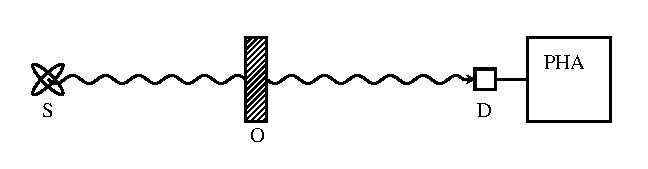
\includegraphics[width=10cm]{2004phys4_3.eps}
\caption{}
\eqname{2004phy4-3}
\end{center}
\end{figure}

\item ガンマ線と物質内の原子の相互作用に関して、主要な過程は3つある。
図\iref{2004phy4-4}(a), (b)にはこのうち、2つを模式的に示し、
また、図\iref{2004phy4-5}のA, B, Cの曲線は、ゲルマニウムに対する、それぞれからの$\mu$への寄与を示す。
図\iref{2004phy4-4}(a)および(b)の過程はそえぞれどう呼ばれているか、またそれぞれが図\iref{2004phy4-5}のA, B, Cのどれに対応するかを答えよ。
さらに、残りの過程の名称を答え、その特徴を示す模式図を図\iref{2004phy4-4}にならって描け。

\begin{figure}[htbp]
\begin{center}
%\includegraphics[scale=0.4]{2004phy4-4.eps}
\includegraphics[width=13cm]{2004phys4_4.eps}
\caption{}
\eqname{2004phy4-4}
\end{center}
\end{figure}

\begin{figure}[htbp]
\begin{center}
%\includegraphics[scale=0.4]{2004phy4-5.eps}
\includegraphics[width=6cm]{2004phys4_5.eps}
\caption{}
\eqname{2004phy4-5}
\end{center}
\end{figure}

\end{enumerate}

\item
原子核や素粒子の崩壊によって放出されるガンマ線に関して以下の設問に答えよ。

\begin{enumerate}
\item
図\iref{2004phy4-6}(a)のように、ある励起した原子核$A^{*}$は、その静止系で、1.4MeVのエネルギーのガンマ線を放出して原子核Aに崩壊する。
実験室で原子核反応により励起した原子核$A^{*}$を生成したところ、実験室系での速さが光速$c$の80\%であった。
図\iref{2004phy4-6}(b)に示すように、実験室系で、崩壊前の$A^{*}$の速度ベクトルの方向に対するガンマ線の放出角度を$\theta_L$とする。$\theta_L$=60°でガンマ線を観測すると、観測されるガンマ線のエネルギーがいくらになるか。有効数字2桁で答えよ。

なお、実験室系の$z$軸方向に速さ$v=\beta c$で静止系が運動しているとき、静止系における4元反変ベクトル$X_\mathrm{C}$と実験室系における4元反変ベクトル$X_\mathrm{L}$は、ローレンツ変換
$$
X_\mathrm{C}=
\left(
\begin{array}{cccc}
\gamma&  0 &0 &-\beta\gamma\\
0&1&0&0\\
0&0&1&0\\
-\beta\gamma &0&0&\gamma
\end{array}
\right)
X_\mathrm{L}
$$
で関連づけられる。ただし、$\gamma=1/\sqrt{1-\beta^2}$である。

\begin{figure}[htbp]
\begin{center}
%\includegraphics[scale=0.4]{2004phy4-6.eps}
\includegraphics[height=5cm]{2004phys4_6.eps}
\caption{}
\eqname{2004phy4-6}
\end{center}
\end{figure}

\item $\pi^0$中間子 (質量$m$) は、おもに2個のガンマ線に崩壊する。実験室でこの崩壊が観測されたとき、2個のガンマ線のそれぞれのエネルギー($E_1$および$E_2$)、2個のガンマ線の方向ベクトルのなす角度$\theta$、および$m$との間にどのような関係が成り立つかを示せ。なお、光速を$c$とせよ。
\end{enumerate}

\end{enumerate}
\end{question}

\begin{answer}{第4問}{}

I. ガンマ線と物質の相互作用について\\
1.物質を$\Delta x$通るとカウント数が$Y\mu \Delta x$減少するので、
\begin{equation}
-\frac{\mathrm{d}Y}{\mathrm{d}X}=\mu Y
\end{equation}
これを初期値$X=0でY=Y_0$の元で解くと、
\begin{align}
Y=Y_0\mathrm{e}^{-\mu x} \\
\therefore \mu =\frac{1}{X} \ln \frac{Y_0}{Y}
\end{align}
\\
2.実験でカウントしているのは、$Y,Y_0$の2つの量であるので、
\begin{align}
\Delta \mu &=\sqrt{(\frac{\partial \mu }{\partial Y}\Delta Y)^2+(\frac{\partial \mu }{\partial Y_0}\Delta Y_0)^2}\\
           &=\frac{1}{X}\sqrt{\frac{1}{Y}+\frac{1}{Y_0}}
\end{align}
ただし、$Y,Y_0$の統計義差をそれぞれ$\sqrt{Y},\sqrt{Y_0}$とした。\\
\\
3. (放射線の実験テキスト参照)\\
(a)コンプトン散乱、曲線はB\\
(b)電子陽電子対生成、曲線はC\\
曲線Aの過程は光電効果であり、図は以下のようになる。
\begin{figure}[h]
\centering
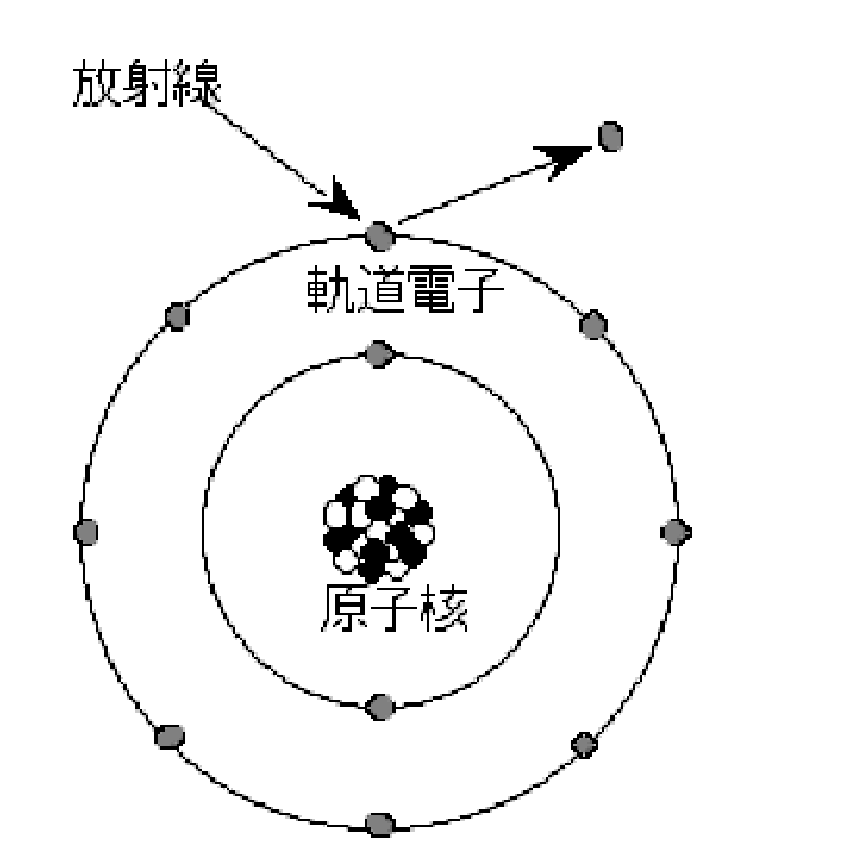
\includegraphics[width=6cm,clip]{2004phy4-1.eps}
\caption{光電効果の模式図}
\end{figure}
\\
\\
II. 粒子崩壊の計算\\
{
%% 1.反変ベクトルとして、四元運動量ベクトル$(E/c,\vec p)$をとる。\\
%% 原子核反応が起こっている平面をxz平面として問題文に与えられたローレンツ変換を用いると、
%% \begin{equation}
%% \begin{pmatrix}E_\mathrm{L}/c \\ p_{\mathrm{L}x} \\ p_{\mathrm{L}y} \\ p_{\mathrm{L}z} \end{pmatrix}=
%% \begin{pmatrix}\gamma & 0 & 0 & -\beta \gamma \\ 0 & 1 & 0 & 0 \\ 0 & 0 & 1 & 0 \\ -\beta \gamma & 0 & 0 & \gamma \end{pmatrix}
%% \begin{pmatrix}E_\mathrm{C}/c \\ p_{\mathrm{C}x} \\ p_{\mathrm{C}y} \\ p_{\mathrm{C}z} \end{pmatrix}.
%% \end{equation}
%% ここでガンマ線は質量ゼロであるので、$E=pc$が成立する。\\
%% また、$p_{Lx} = p_L \cos \theta_L,p_{Lz} = p_L \sin \theta_L$であるとする。\\
%% $\theta_C=60^\circ ,E_C=1.4\mbox{MeV},\beta =0.8,\gamma =\frac{1}{\sqrt{1-\beta ^2}}=\frac{1}{0.6}$として解くと、
%% $E_L=0.6$MeV を得る。\\
  %% <modified date="20120731" auth="Koichi Murase">
  \noindent 1.
  反応が起こっている平面を $x$-$z$ 平面とし、
  図の右方向を $z$ 軸とし、図の上方向を $x$ 軸とする。
  ガンマ線は質量ゼロなので $E_\mathrm{L}=p_\mathrm{L}c$ である。
  従って、$p_{\mathrm{L}z} = p_{\mathrm{L}}\cos\theta_\mathrm{L} = (E_\mathrm{L}/c)\cdot\cos\theta_\mathrm{L} $ となる。
  ガンマ線の四元運動量 $(E/c,\, \vec p)$ に対して
  問題文に与えられたローレンツ変換を用いると、
  \begin{eqnarray}
    E_\mathrm{C}/c &=& \gamma (E_\mathrm{L}/c - \beta p_{\mathrm{L}z}) = \gamma (E_\mathrm{L}/c -\beta \cos\theta_\mathrm{L} E_\mathrm{L}/c),\\
    E_\mathrm{C} &=& E_\mathrm{L} \gamma(1 -\beta \cos\theta_\mathrm{L} ).
  \end{eqnarray}
  これに $\theta_\mathrm{L}=60^\circ$, $E_\mathrm{C}$=1.4 MeV, $\beta$=0.8, $\gamma =1/\sqrt{1-\beta ^2}=1/0.6$ を代入すると
  $E_\mathrm{L}$=1.4 MeV が得られる。
  %% </modified>
}\\
2.\begin{figure}[h]
\centering
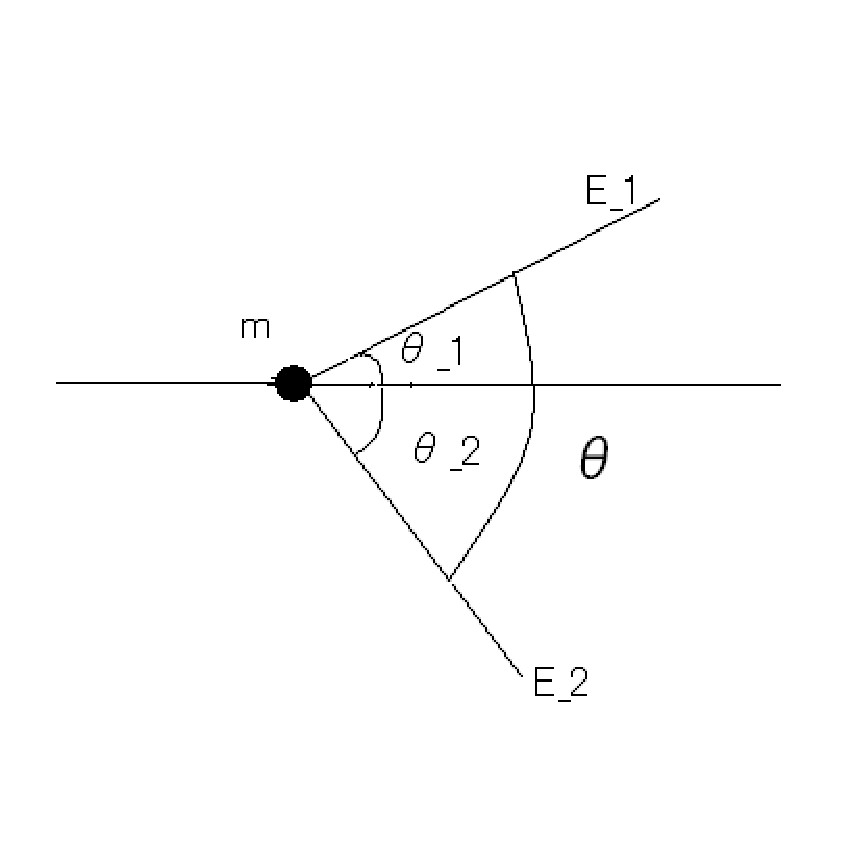
\includegraphics[width=6cm,clip]{2004phy4-2.eps}
\end{figure}
 $\pi ^0$ 中間子の実験室系での速度を$\beta c$とする。$E_1=p_1c,E_2=p_2c$として、運動量の保存より
\begin{eqnarray}
m\gamma \beta c&=&p_1\cos \theta _1+p_2\cos \theta _2 \eqname{eq:siki1}\\
0&=&p_1\sin \theta _1-p_2\sin \theta _2 \eqname{eq:siki2}
\end{eqnarray}
$式(\eqhref{eq:siki1})\times\sin \theta _1-式(\eqhref{eq:siki2})\times\sin \theta _2$より
\begin{equation}
m\gamma \beta \sin \theta _1c=p_2\sin \theta \eqname{eq:siki3}
\end{equation}
$式(\eqhref{eq:siki1})\times\cos \theta _1+式(\eqhref{eq:siki2})\times\sin \theta _1$より
\begin{equation}
m\gamma \beta \cos \theta _1c=p_1+p_2 \cos \theta \eqname{eq:siki4}
\end{equation}
式 (\eqhref{eq:siki3}) と式 (\eqhref{eq:siki4}) を辺々2乗して足すと、
\begin{eqnarray}
(m\gamma \beta c)^2 &=& {p_1}^2+{p_2}^2+2 p_1 p_2 \cos \theta \\
                   &=& (\frac{E_1}{c})^2+(\frac{E_2}{c})^2+2\frac{E_1E_2}{c^2}\cos \theta \eqname{eq:siki5}
\end{eqnarray}
ここで$\beta \gamma $は、エネルギー保存則より
\begin{equation}
(m\gamma \beta c^2)^2+(m c^2)^2=(E_1+E_2)^2 \eqname{eq:siki6}
\end{equation}
をみたすので、式 (\eqhref{eq:siki5}) (\eqhref{eq:siki6}) より
\begin{equation}
2E_1 E_2(1-\cos \theta )=(mc^2)^2
\end{equation}
を得る。 
\end{answer}
\end{document}
